\chapter{Tests and results}
\label{cha:4}
In this last chapter we discuss the results of the tests, focusing on some particular metrics in relation to the specifications given at the beginning of the project. For the environment of testing we created a small network of virtual machines that could properly stress testing a Mongo database and give a more realistic feedback in terms of network overhead.
Proceeding through the chapter, we deeply explain each metric analyzed and compare the results between different test cases.

\section{Environment of testing}
\label{sec:1}
Since multithreading inside the Java Virtual Machine is quite expensive in terms of CPU and memory usage, it was not possible to launch more than 8 threads from a single machine. 
The environment of testing is a small LAN of virtual and physical machines connected and controlled in SSH \footnote{http://www.cisco.com/c/en/us/about/press/internet-protocol-journal/back-issues/table-contents-46/124-ssh.html} using Putty from a laptop.
The following virtual machines are part of the evironment: 
\begin{itemize}
	\item \textit{vm-mondb} running a Mongo node as Master with the following hardware specifications - CPU: Intel i7 Quadcore @2400Mhz, RAM: 4Gb, HDD: 30Gb.
	\item \textit{vm-mondb2} running a Mongo secondary node as Slave with the following hardware specifications - CPU: Intel i7 Quadcore @2400Mhz, RAM: 4Gb, HDD: 30Gb.
	\item \textit{vm01-st} and \textit{vm02-st} running the MongoDB Resource standalone module with the following specifications - CPU: QEMU Quadcore @1800Mhz, RAM: 4Gb, HDD: 6,7Gb.
	\item \textit{vm03-st} running the MongoDB Resource standalone module with the following specifications - CPU: QEMU Dualcore @1800Mhz, RAM: 4Gb, HDD: 5,3Gb.
\end{itemize}
\begin{figure}[H]
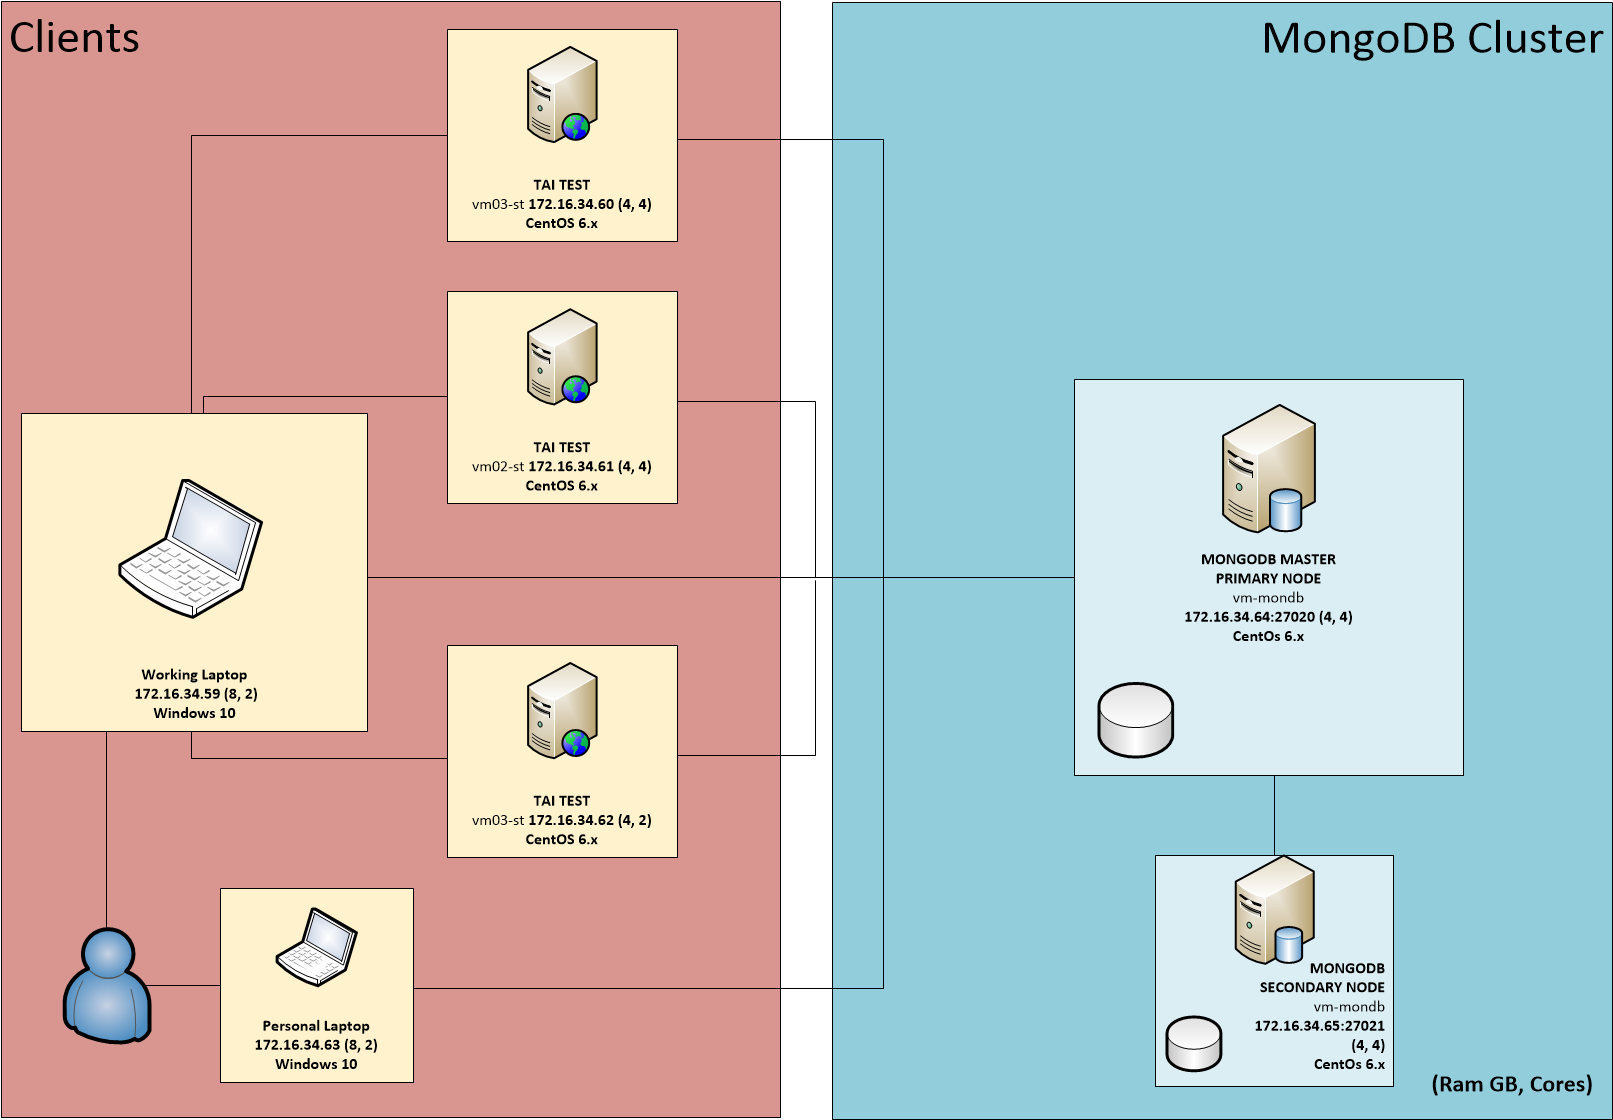
\includegraphics[scale=0.5]{my_architecture.png}
\centering
\caption{Representation of the environment of testing.}
\end{figure}
Every virtual machine was running a Linux distribution, CentOS, and they were controlled simultaneously using Putty. On every  client machine an instance of the MongoDB Resource Module was running from the Linux shell with same test configuration.
On the machines hosting the Mongo nodes, Mongo had two different configurations: 


The primary node was running a \textit{mongod} \footnote{See section 2.5} instance with 2 different \textit{config servers} \footnote{See section 2.6}. This configuration allowed to quickly switch from a single- node configuration to a double-node (or more) configuration.
\begin{lstlisting}
# mongod.conf

# for documentation of all options, see:
#   http://docs.mongodb.org/manual/reference/configuration-options/

# where to write logging data.
systemLog:
  destination: file
  logAppend: true
  path: /var/log/mongodb/mongod_configsvr.log

# Where and how to store data.
storage:
  dbPath: /var/lib/mongo
  journal:
    enabled: true
#  engine:
#  mmapv1:
#  wiredTiger:

# how the process runs
processManagement:
  fork: true  # fork and run in background
  pidFilePath: /var/run/mongodb/mongod_configsvr.pid  # location of pidfile
  #pidFilePath: /var/run/mongodb/mongod_configsvr2.pid # location of pidfile for 2 nodes configuration

# network interfaces
net:
  port: 27021
#  bindIp: 127.0.0.1  # Listen to local interface only, comment to listen on all interfaces.

#security:

#operationProfiling:

#replication:

#sharding:

## Enterprise-Only Options

#auditLog:

#snmp:
\end{lstlisting}

\newpage
The secondary node was running a \textit{mongos} instance instead, that automatically connects to the primary node in case the configuration for 2 nodes is set. \textit{Replica Set} was not enabled because in a benchmark test it would only affect performance and it is usually a production choice where it could provide consistency and durability of the data.

\begin{lstlisting}
# mongos.conf

# for documentation of all options, see:
#   http://docs.mongodb.org/manual/reference/configuration-options/

# where to write logging data.
systemLog:
  destination: file
  logAppend: true
  path: /var/log/mongodb/mongos.log

# Where and how to store data.
#storage:
#  dbPath: /var/lib/mongo
#  journal:
#    enabled: true
#  engine:
#  mmapv1:
#  wiredTiger:

# how the process runs
processManagement:
  fork: true  # fork and run in background
  pidFilePath: /var/run/mongodb/mongos.pid  # location of pidfile

# network interfaces
net:
  port: 27020
#  bindIp: 127.0.0.1  # Listen to local interface only, comment to listen on all interfaces.


#security:

#operationProfiling:

#replication:

sharding:
  configDB: vm-mondb:27020

## Enterprise-Only Options

#auditLog:

#snmp:
\end{lstlisting}

 
\section{Test cases and setup}
\label{sec:2}
Basically, three different tests have run with both configurations of Mongo (with one and with two nodes). 
The plan was to perform tests of increasing complexity and data workload to analyze the differences between their results and to  understand how Mongo reacts under stressing conditions.
\begin{itemize}
	\item \textit{First Type} : this type tests every main feature of the software and  give a first overview on Mongo performance in normal conditions.
	\item \textit{Second Type} : this type heavily stresses Mongo with multiple parallel connections and inserting at maximum speed 2.000.000 of documents. It was used to analyze Mongo scalability rate from 1 to 2 nodes.
	\item \textit{Third Type} : this type has the same stressing purpose as Second Type with identical configuration, in addition it executes a specific search using as parameter a random number assigned to each document. This query is executed every 10 seconds for 750 times returning an increasing set of matching documents.
\end{itemize}


\section{Gathering data}
\label{sec:3}
In this phase all data spread across 4 different instances of MongoDB Resource Module have been gathered using the UI Module on a laptop connected to the LAN.
In the meanwhile on another laptop the UI Module plotted all the data of its MongoDB Resource Module instance. It was not possible to plot the results from the virtual machines because their data did not pass through the Angular module dedicated to this function. This is unfortunately a limitation of the actual implementation of the software.
All the metrics tables and the graphs plotted by the UI module were printed on .jpeg files and then inserted into an Excel Spreadsheet where there is a page for each test. All the averages from all the machines for each test have been calculated using Excel inside the relative page and then linked to the summary page to compare all the tests. Any plotted graph has been linked into those pages but not into the summary page to allow a clean presentation to any reader.
This Excel Spreadsheet \footnote{https://drive.google.com/open?id=0B1IlD5PLfM8\_LTY5QjVXR0R3SE0} is freely available for consultation. 
It is possible to read all the data retrieved from the tests, but as they are quite a lot and eventually confusing, only the most interesting and meaningful are analyzed in the following sections. For more details, all readers are free to consult that file.

\section{Analyzing results}
\label{sec:4}

\subsection{Description of the metrics analyzed}
Before going deeper into the analysis, we are going to explain which metrics have been analyzed and how they have been calculated:
\begin{itemize}
	\item \textit{Average Put Time / Average Get Time} : respectively average time of insertion and retrieve of a document into/from the database.
	\item \textit{Max Put Time / Min Put Time} : respectively maximum and minimum time of insertion into the database.
	\item \textit{Max Get Time / Min Get Time} : respectively maximum and minimum time of insertion into the database.
	\item \textit{Throughput} : total amount of operations (put and get) divided by the total time needed to complete the workload of the test.
	\item \textit{Failure Rate} :total number of failed operations (that returned an exception) over the total number of operations performed.
\end{itemize}
There are some approximations in the metrics presented in the \textit{Summary page} of the Excel Spreadsheet due to the high number of running threads on different machines:
\begin{itemize}
	\item \textit{Test Duration} : it refers to the time taken by the slowest machine of each test to complete the workload. It is not the time used to calculate \textit{Throughput}.
	\item \textit{Avg Put/Get Times} : those are the average of the Average Put/Get Times calculated on each machine in a test.
	\item \textit{Max and Min Put/Get Times} : those are the maximum and the minimum put/get times overall of a test.
	\item \textit{Throughput} : it is the average the Throughput calculated on each machine in a test, so for example if a machine took time "T" to perform "n" operations on "i" machines, the formula to obtain this final throughput is: 
\[Throughput = \frac{\sum_{0}^{i}\frac{n_{i}}{T_{i}}}{i}\]

\end{itemize}
Now that we have defined the meaning of those values, we can analyze the most significant tests.
\subsection{Analyzed Tests}
A total number of 10 tests have been performed using \textsc{MongoDb Performance}, but some of them failed or were not relevant.
We take in account only \textit{Test1}, \textit{Test4}, \textit{Test6} and \textit{Test10} because for the following reasons the others cannot be relevant.
Tests from 1 to 3 are not real load tests, they did not “stress” Mongo at all, so only one of them is presented as example.
\textit{Test5} suffered the desynchronization of the OS time clock of a Mongo node with the other of about half an hour, and since Mongo assigns \textit{\_id} using timestamp of the machine and then balances documents between the nodes on a Shard Key that includes by default \textit{\_id} \footnote{This is a good reason to specify a Shard Key on a different field.}, the two nodes lost performance and data were divided approximately 60\% on the first node and 40\% on the second node. 
Each test  took some hours to run, some of them have scheduled for automatic launch during the night to save time.
For unknown reasons, \textit{Test7} and  \textit{Test9} were incomplete due to an interruption of alimentation of the laptop used to plot data \footnote{The laptop itself was running threads that unfortunately stopped performing operations on Mongo}.
As last, we can ignore \textit{Test8} as the complexity of the query used to stress Mongo was too low with to affect the database performance, resulting in a test similar to \textit{Test4}.
Anyway, all machines that completely performed their workload have been kept in the analysis because there was no time to repeat the tests before the presentation scheduled date and they still confirmed Mongo efficient performance \footnote{Data were partially comparable}.

\subsection{Results}
the table gathers the most relevant results from the analysis spreadsheet, cleaned from all unnecessary columns and details.
%\begin{figure}[H]
%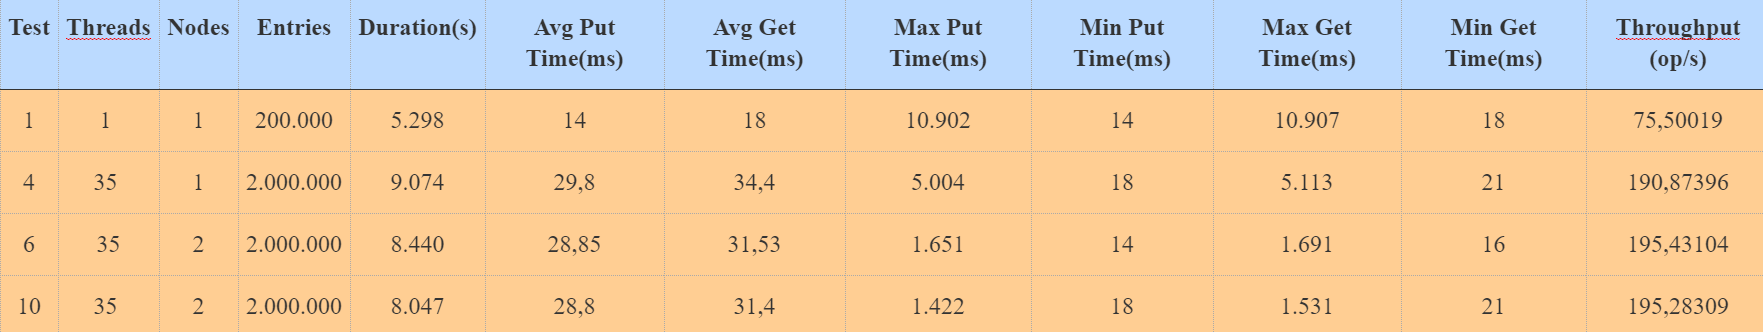
\includegraphics[scale=0.3]{table.png}
%\centering
%\caption{Summary of the analyzed metrics.}
%\end{figure}
\begin{table}[H]
\centering
\label{my-label}
\begin{tabular}{@{}ccccccc@{}}
\toprule
\rowcolor[HTML]{BBDAFF} 
Test & Threads & Nodes & Entries & Duration(s) & Avg Put Time(ms) & Avg Get Time(ms) \\ \midrule
\rowcolor[HTML]{FFCC67} 
1 & 1 & 1 & 200.000 & 5.298 & 14 & 18 \\
\rowcolor[HTML]{FFCC67} 
4 & 35 & 1 & 2.000.000 & 9.074 & 29,8 & 34,4 \\
\rowcolor[HTML]{FFCC67} 
6 & 35 & 2 & 2.000.000 & 8.440 & 28,85 & 31,53 \\
\rowcolor[HTML]{FFCC67} 
10 & 35 & 2 & 2.000.000 & 8.047 & 28,8 & 31,4 \\ \bottomrule
\end{tabular}
\end{table}

\begin{table}[H]
\centering
\begin{tabular}{@{}cccccc@{}}
\toprule
\rowcolor[HTML]{BBDAFF} 
Test & \begin{tabular}[c]{@{}c@{}}Max\\  Put Time(ms)\end{tabular} & \begin{tabular}[c]{@{}c@{}}Min\\ Put Time(ms)\end{tabular} & \begin{tabular}[c]{@{}c@{}}Max \\ Get Time(ms)\end{tabular} & \begin{tabular}[c]{@{}c@{}}Min \\ Get Time(ms)\end{tabular} & Throughput(op/s) \\ \midrule
\rowcolor[HTML]{FFCC67} 
1 & 10.902 & 14 & 10.907 & 18 & 75,50019 \\
\rowcolor[HTML]{FFCC67} 
4 & 5.004 & 18 & 5.113 & 21 & 190,87396 \\
\rowcolor[HTML]{FFCC67} 
6 & 1.651 & 14 & 1.691 & 16 & 195,43104 \\
\rowcolor[HTML]{FFCC67} 
10 & 1.422 & 18 & 1.531 & 21 & 195,28309 \\ \bottomrule
\end{tabular}
\caption{Summary of the analyzed metrics.}
\label{my-label}
\end{table}

All of those tests run with a 50 – 50 workload type, meaning that half of the operation were \textit{put} operations and the other half \textit{get} operations, for example having 200.000 entries means that 400.000 operations are performed during the test.
There are three different typologies of test \footnote{See section 4.2} so we analyze at least one test for each typology: Test 1 belongs to the First Type and so it was just a functional test with a small workload performed on a Mongo database with 1 node. It obtained a \textit{Max Put Time} and a \textit{Max Get Time} of more than 10 seconds, but some considerations should be taken in account:
\begin{itemize}
	\item Each \textit{get} operation happen after a \textit{put} operation, so it’s reasonable to assume that \textit{Max Get Time} of 10.907 ms is  the result of \textit{Max Put Time} + 5 ms \footnote{In simple words, get time is anyway acceptable.}.
	\item \textit{Avg Put Time} and \textit{Avg Get Time} stay on really low values, respectively 14 ms and 18 ms, that in first place satisfies the customer requisite of 2 seconds to retrieve data from the database. In second place it means that since they are average values and they do not appear to be affected by \textit{Max Put/Get Time},  those “worse" cases are just a very few over the total operations performed.
\end{itemize}
\textit{Test 4} and \textit{Test 6} belong to the Second Type, they are stress tests performed with same configuration. In total they execute 2 million entries \footnote {4.000.000 operations with this type of workload} running 35 parallel threads with all virtual machines available. The only difference between them is that \textit{Test 4} runs on a Mongo database with 1 node while \textit{Test 6} runs on a Mongo database with 2 nodes and a Shard Key on the \textit{\_id} field.
It is possible to appreciate how Mongo scales well horizontally by adding nodes to its configuration. First, \textit{Duration} is a bit shorter and \textit{Avg Put/Get Times} are slightly better. Most important is that with multiple nodes none of the operations took more than 1,7 seconds to execute. This means that Mongo manages concurrency more efficiently with more nodes, that is what we expected in terms of scalability and distribution of data. In the average, Mongo performed 5 more operations each second using 2 nodes.
At last, \textit{Test 10} belongs to Third Type and was performed with the same configuration as \textit{Test 6} \footnote{35 threads, 2 millions entries, 2 nodes}, but with an additional single field index on the field \textit{rIndex}, containing a random generated number between 0 and 3.000.000.
During this test along with other operations, a "Complex Query" have been automatically executed every 10 seconds for a total of 750 times on the database. This query takes a random number  R between 0 and 2.999.900 and retrieves all the documents having  \textit{rIndex} in the set \{R , R+100\}.
With the progressive increase of \textit{n} as total number of documents in the database, the query takes increasing average time to execute. 
The following chart represents all execution times of the query over the total executions.
\begin{figure}[H]
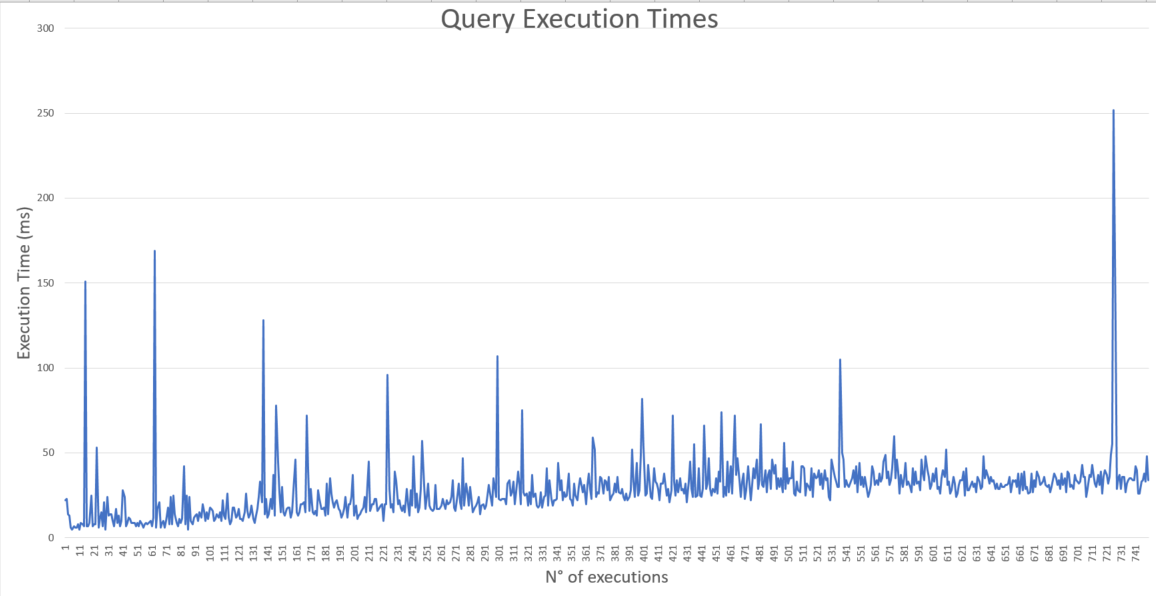
\includegraphics[scale=0.55]{exec_times_new.png}
\centering
\caption{Query execution times.}
\end{figure}
The average time of execution appears to increase following a logarithmic curve and this is consistent with MongoDB implementation of data structures research .
In fact, Mongo uses B+ Trees as data structure and consequently the complexity of a \textit{find( )} function is O(logn).
This great result obviously has a cost: \textit{Min Put/Get Times} have a worse performance in our benchmark  because of the secondary index on \textit{rIndex}. 
Even if  there are not evident differences in the \textit{Avg Put/Get Times}, the \textit{Throughput} slightly decreases and probably with a higher number of documents it would become more perceptible.
In a production software anyway there are usually less insert operations than get operations, therefore using indexes with a small cost on the insertion time is completely worth the increase of reading speed.
In conclusion, low average times to perform query data, no data loss \footnote{0\% failure rate in every test } and an appreciable scalability even using  “weak” hardware specifications, MongoDB confirms to be a choice that perfectly fits the needs of our commission.
\section{Comparing results with other benchmarks}
\label{sec:5}
In the spreadsheet summary, there are also some results of tests performed by other two companies with better hardware components to support bigger workloads. Those benchmarks have been used in the beginning of the project as inspiration and also as first overview on Mongo and its performance with a proper hardware.
Unfortunately they cannot be compared with our results in the end.
The main problem with many benchmarks available on the web is that they are often committed, or even performed, by companies that own a NoSQL solution to show its streght over the others.
This lead to a problem of advertising part and to specific benchmark tests made within ad-hoc situations in which a certain NoSQL database performs at its best.
Anyway, most of the benchmarks agree that the NoSQL database that actually gains most from Horizontal Scalability is Apache Cassandra thanks to its Key-Value implementation.
Other NoSQL solutions are better in some particular use cases, consequently when a company decides to migrate to a new NoSQL solutions  it should try to find the one that fit its specific needs.
